\documentclass{ximera}

%\usepackage{todonotes}

\newcommand{\todo}{}

\usepackage{esint} % for \oiint
\ifxake%%https://math.meta.stackexchange.com/questions/9973/how-do-you-render-a-closed-surface-double-integral
\renewcommand{\oiint}{{\large\bigcirc}\kern-1.56em\iint}
\fi


\graphicspath{
  {./}
  {ximeraTutorial/}
  {basicPhilosophy/}
  {functionsOfSeveralVariables/}
  {normalVectors/}
  {lagrangeMultipliers/}
  {vectorFields/}
  {greensTheorem/}
  {shapeOfThingsToCome/}
  {dotProducts/}
  {partialDerivativesAndTheGradientVector/}
  {../productAndQuotientRules/exercises/}
  {../normalVectors/exercisesParametricPlots/}
  {../continuityOfFunctionsOfSeveralVariables/exercises/}
  {../partialDerivativesAndTheGradientVector/exercises/}
  {../directionalDerivativeAndChainRule/exercises/}
  {../commonCoordinates/exercisesCylindricalCoordinates/}
  {../commonCoordinates/exercisesSphericalCoordinates/}
  {../greensTheorem/exercisesCurlAndLineIntegrals/}
  {../greensTheorem/exercisesDivergenceAndLineIntegrals/}
  {../shapeOfThingsToCome/exercisesDivergenceTheorem/}
  {../greensTheorem/}
  {../shapeOfThingsToCome/}
  {../separableDifferentialEquations/exercises/}
  {vectorFields/}
}

\newcommand{\mooculus}{\textsf{\textbf{MOOC}\textnormal{\textsf{ULUS}}}}

\usepackage{tkz-euclide}
\usepackage{tikz}
\usepackage{tikz-cd}
\usetikzlibrary{arrows}
\tikzset{>=stealth,commutative diagrams/.cd,
  arrow style=tikz,diagrams={>=stealth}} %% cool arrow head
\tikzset{shorten <>/.style={ shorten >=#1, shorten <=#1 } } %% allows shorter vectors

\usetikzlibrary{backgrounds} %% for boxes around graphs
\usetikzlibrary{shapes,positioning}  %% Clouds and stars
\usetikzlibrary{matrix} %% for matrix
\usepgfplotslibrary{polar} %% for polar plots
\usepgfplotslibrary{fillbetween} %% to shade area between curves in TikZ
%\usetkzobj{all}
\usepackage[makeroom]{cancel} %% for strike outs
%\usepackage{mathtools} %% for pretty underbrace % Breaks Ximera
%\usepackage{multicol}
\usepackage{pgffor} %% required for integral for loops



%% http://tex.stackexchange.com/questions/66490/drawing-a-tikz-arc-specifying-the-center
%% Draws beach ball
\tikzset{pics/carc/.style args={#1:#2:#3}{code={\draw[pic actions] (#1:#3) arc(#1:#2:#3);}}}



\usepackage{array}
\setlength{\extrarowheight}{+.1cm}
\newdimen\digitwidth
\settowidth\digitwidth{9}
\def\divrule#1#2{
\noalign{\moveright#1\digitwidth
\vbox{\hrule width#2\digitwidth}}}




% \newcommand{\RR}{\mathbb R}
% \newcommand{\R}{\mathbb R}
% \newcommand{\N}{\mathbb N}
% \newcommand{\Z}{\mathbb Z}

\newcommand{\sagemath}{\textsf{SageMath}}


%\renewcommand{\d}{\,d\!}
%\renewcommand{\d}{\mathop{}\!d}
%\newcommand{\dd}[2][]{\frac{\d #1}{\d #2}}
%\newcommand{\pp}[2][]{\frac{\partial #1}{\partial #2}}
% \renewcommand{\l}{\ell}
%\newcommand{\ddx}{\frac{d}{\d x}}

% \newcommand{\zeroOverZero}{\ensuremath{\boldsymbol{\tfrac{0}{0}}}}
%\newcommand{\inftyOverInfty}{\ensuremath{\boldsymbol{\tfrac{\infty}{\infty}}}}
%\newcommand{\zeroOverInfty}{\ensuremath{\boldsymbol{\tfrac{0}{\infty}}}}
%\newcommand{\zeroTimesInfty}{\ensuremath{\small\boldsymbol{0\cdot \infty}}}
%\newcommand{\inftyMinusInfty}{\ensuremath{\small\boldsymbol{\infty - \infty}}}
%\newcommand{\oneToInfty}{\ensuremath{\boldsymbol{1^\infty}}}
%\newcommand{\zeroToZero}{\ensuremath{\boldsymbol{0^0}}}
%\newcommand{\inftyToZero}{\ensuremath{\boldsymbol{\infty^0}}}



% \newcommand{\numOverZero}{\ensuremath{\boldsymbol{\tfrac{\#}{0}}}}
% \newcommand{\dfn}{\textbf}
% \newcommand{\unit}{\,\mathrm}
% \newcommand{\unit}{\mathop{}\!\mathrm}
% \newcommand{\eval}[1]{\bigg[ #1 \bigg]}
% \newcommand{\seq}[1]{\left( #1 \right)}
% \renewcommand{\epsilon}{\varepsilon}
% \renewcommand{\phi}{\varphi}


% \renewcommand{\iff}{\Leftrightarrow}

% \DeclareMathOperator{\arccot}{arccot}
% \DeclareMathOperator{\arcsec}{arcsec}
% \DeclareMathOperator{\arccsc}{arccsc}
% \DeclareMathOperator{\si}{Si}
% \DeclareMathOperator{\scal}{scal}
% \DeclareMathOperator{\sign}{sign}


%% \newcommand{\tightoverset}[2]{% for arrow vec
%%   \mathop{#2}\limits^{\vbox to -.5ex{\kern-0.75ex\hbox{$#1$}\vss}}}
% \newcommand{\arrowvec}[1]{{\overset{\rightharpoonup}{#1}}}
% \renewcommand{\vec}[1]{\arrowvec{\mathbf{#1}}}
% \renewcommand{\vec}[1]{{\overset{\boldsymbol{\rightharpoonup}}{\mathbf{#1}}}}

% \newcommand{\point}[1]{\left(#1\right)} %this allows \vector{ to be changed to \vector{ with a quick find and replace
% \newcommand{\pt}[1]{\mathbf{#1}} %this allows \vec{ to be changed to \vec{ with a quick find and replace
% \newcommand{\Lim}[2]{\lim_{\point{#1} \to \point{#2}}} %Bart, I changed this to point since I want to use it.  It runs through both of the exercise and exerciseE files in limits section, which is why it was in each document to start with.

% \DeclareMathOperator{\proj}{\mathbf{proj}}
% \newcommand{\veci}{{\boldsymbol{\hat{\imath}}}}
% \newcommand{\vecj}{{\boldsymbol{\hat{\jmath}}}}
% \newcommand{\veck}{{\boldsymbol{\hat{k}}}}
% \newcommand{\vecl}{\vec{\boldsymbol{\l}}}
% \newcommand{\uvec}[1]{\mathbf{\hat{#1}}}
% \newcommand{\utan}{\mathbf{\hat{t}}}
% \newcommand{\unormal}{\mathbf{\hat{n}}}
% \newcommand{\ubinormal}{\mathbf{\hat{b}}}

% \newcommand{\dotp}{\bullet}
% \newcommand{\cross}{\boldsymbol\times}
% \newcommand{\grad}{\boldsymbol\nabla}
% \newcommand{\divergence}{\grad\dotp}
% \newcommand{\curl}{\grad\cross}
%\DeclareMathOperator{\divergence}{divergence}
%\DeclareMathOperator{\curl}[1]{\grad\cross #1}
% \newcommand{\lto}{\mathop{\longrightarrow\,}\limits}

% \renewcommand{\bar}{\overline}

\colorlet{textColor}{black}
\colorlet{background}{white}
\colorlet{penColor}{blue!50!black} % Color of a curve in a plot
\colorlet{penColor2}{red!50!black}% Color of a curve in a plot
\colorlet{penColor3}{red!50!blue} % Color of a curve in a plot
\colorlet{penColor4}{green!50!black} % Color of a curve in a plot
\colorlet{penColor5}{orange!80!black} % Color of a curve in a plot
\colorlet{penColor6}{yellow!70!black} % Color of a curve in a plot
\colorlet{fill1}{penColor!20} % Color of fill in a plot
\colorlet{fill2}{penColor2!20} % Color of fill in a plot
\colorlet{fillp}{fill1} % Color of positive area
\colorlet{filln}{penColor2!20} % Color of negative area
\colorlet{fill3}{penColor3!20} % Fill
\colorlet{fill4}{penColor4!20} % Fill
\colorlet{fill5}{penColor5!20} % Fill
\colorlet{gridColor}{gray!50} % Color of grid in a plot

\newcommand{\surfaceColor}{violet}
\newcommand{\surfaceColorTwo}{redyellow}
\newcommand{\sliceColor}{greenyellow}




\pgfmathdeclarefunction{gauss}{2}{% gives gaussian
  \pgfmathparse{1/(#2*sqrt(2*pi))*exp(-((x-#1)^2)/(2*#2^2))}%
}


%%%%%%%%%%%%%
%% Vectors
%%%%%%%%%%%%%

%% Simple horiz vectors
\renewcommand{\vector}[1]{\left\langle #1\right\rangle}


%% %% Complex Horiz Vectors with angle brackets
%% \makeatletter
%% \renewcommand{\vector}[2][ , ]{\left\langle%
%%   \def\nextitem{\def\nextitem{#1}}%
%%   \@for \el:=#2\do{\nextitem\el}\right\rangle%
%% }
%% \makeatother

%% %% Vertical Vectors
%% \def\vector#1{\begin{bmatrix}\vecListA#1,,\end{bmatrix}}
%% \def\vecListA#1,{\if,#1,\else #1\cr \expandafter \vecListA \fi}

%%%%%%%%%%%%%
%% End of vectors
%%%%%%%%%%%%%

%\newcommand{\fullwidth}{}
%\newcommand{\normalwidth}{}



%% makes a snazzy t-chart for evaluating functions
%\newenvironment{tchart}{\rowcolors{2}{}{background!90!textColor}\array}{\endarray}

%%This is to help with formatting on future title pages.
\newenvironment{sectionOutcomes}{}{}



%% Flowchart stuff
%\tikzstyle{startstop} = [rectangle, rounded corners, minimum width=3cm, minimum height=1cm,text centered, draw=black]
%\tikzstyle{question} = [rectangle, minimum width=3cm, minimum height=1cm, text centered, draw=black]
%\tikzstyle{decision} = [trapezium, trapezium left angle=70, trapezium right angle=110, minimum width=3cm, minimum height=1cm, text centered, draw=black]
%\tikzstyle{question} = [rectangle, rounded corners, minimum width=3cm, minimum height=1cm,text centered, draw=black]
%\tikzstyle{process} = [rectangle, minimum width=3cm, minimum height=1cm, text centered, draw=black]
%\tikzstyle{decision} = [trapezium, trapezium left angle=70, trapezium right angle=110, minimum width=3cm, minimum height=1cm, text centered, draw=black]


\title{Discontinuity}

\begin{document}

\begin{abstract}
sudden breaks
\end{abstract}
\maketitle



The graphs we have seen so far clearly show all kinds of breaks.  The function represented by the graph below is experiencing some drastic behavior around some individual domain numbers.  Let's examine some of these breaks and classify them into a few types.







\subsection*{Basic Types of Breaks}

A quick review of graphs seen so far in this course shows there are three basic types of breaks.




\begin{image}
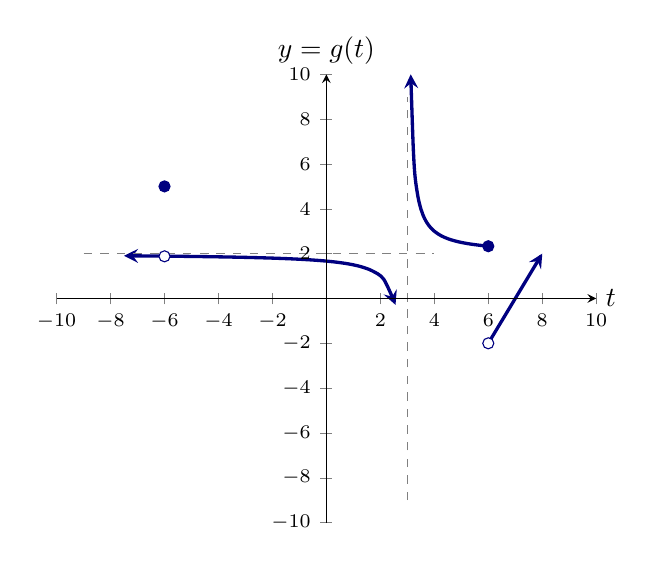
\begin{tikzpicture}
     \begin{axis}[
            	domain=-10:10, ymax=10, xmax=10, ymin=-10, xmin=-10,
            	axis lines =center, xlabel=$t$, ylabel={$y=g(t)$},
                ytick={-10,-8,-6,-4,-2,2,4,6,8,10},
                xtick={-10,-8,-6,-4,-2,2,4,6,8,10},
                yticklabels={$-10$,$-8$,$-6$,$-4$,$-2$,$2$,$4$,$6$,$8$,$10$}, 
                xticklabels={$-10$,$-8$,$-6$,$-4$,$-2$,$2$,$4$,$6$,$8$,$10$},
                ticklabel style={font=\scriptsize},
            	every axis y label/.style={at=(current axis.above origin),anchor=south},
            	every axis x label/.style={at=(current axis.right of origin),anchor=west},
            	axis on top,
          		]

        
        \addplot [draw=penColor, very thick, smooth, domain=(-7.5:3), <->] {1/(x-3) + 2};
        \addplot [draw=penColor, very thick, smooth, domain=(3:6), <-] {1/(x-3) + 2};
        \addplot [draw=penColor, very thick, smooth, domain=(6:8), ->] {2*x-14};

        \addplot [line width=0.5, gray, dashed,samples=100,domain=(-9:9)] ({3},{x});
        \addplot [line width=0.5, gray, dashed,samples=100,domain=(-9:4)] ({x},{2});

        \addplot[color=penColor,fill=penColor,only marks,mark=*] coordinates{(-6,5)};
        \addplot[color=penColor,fill=white,only marks,mark=*] coordinates{(-6,1.88)};
        \addplot[color=penColor,fill=penColor,only marks,mark=*] coordinates{(6,2.33)};
        \addplot[color=penColor,fill=white,only marks,mark=*] coordinates{(6,-2)};

    \end{axis}



\end{tikzpicture}
\end{image}



\begin{itemize}
\item \textbf{\textcolor{blue!75!black}{Removeable:}}  The graph above has a very subtle break at $t=-6$. The graph is almost one piece, except one point has been shifted up. This type of break gets the name \textit{removeable}, because you could remove the break by just sliding that point back in place. \\

\item \textbf{\textcolor{blue!75!black}{Asymptotic:}} The break at $t=3$ is not subtle at all.  One side is heading up to infinty and the other side is heading down to negative infinity.  You can't get a bigger break than that. Graphically, the asymptote is communicating this behavior, hence, the break is called an \textit{asymptotic} break. \\

\item \textbf{\textcolor{blue!75!black}{Jump:}} The break at $t=6$ is called a \textit{jump}, because the graph makes a sudden vertical jump from one location to another location.
\end{itemize}


In all three cases, the graph experiences a sudden vertical movement.  This sudden vertical movement may not be predictable from the points leading up to the sudden movement.








\subsection*{Discontinuities}
One of the strongest purposes of mathematics is simply description and communication.  We like mathematics to be explicit and exact, which requires the support of lots of specific language and notation. We call this \textbf{\textcolor{purple!85!blue}{rigor}}. As we investigate breaks in the graphs of functions, we want language that is explicit, so that we can clearly communicate about the underlying function behavior.

With this in mind, let's compare the following two graphs.


\begin{image}
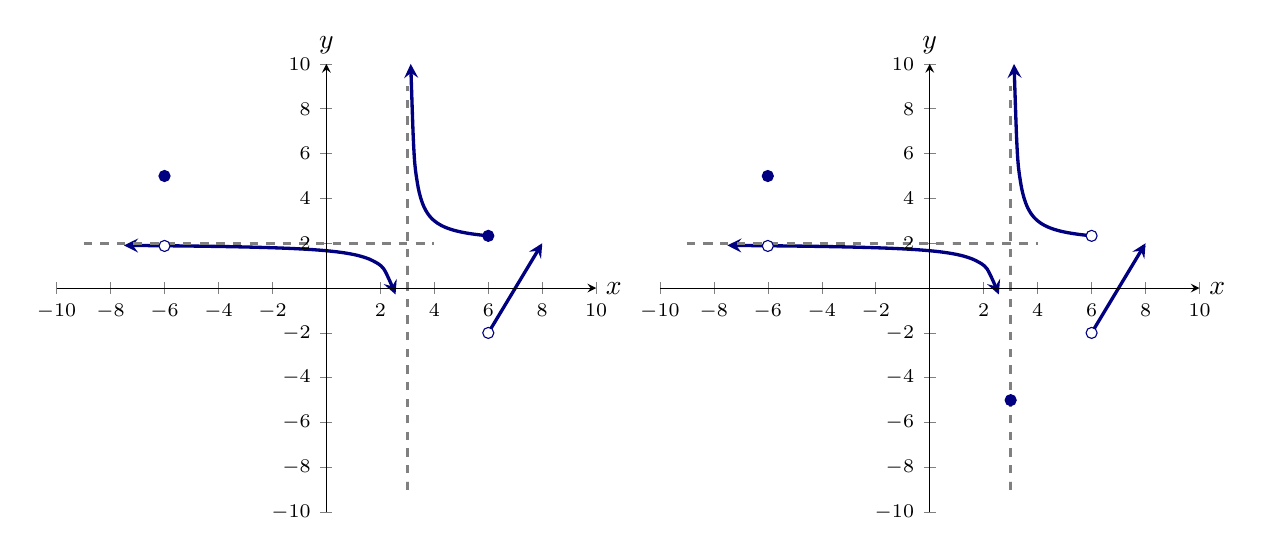
\begin{tikzpicture}
    \begin{axis}[name = without,
            	domain=-10:10, ymax=10, xmax=10, ymin=-10, xmin=-10,
            	axis lines =center, xlabel=$x$, ylabel=$y$,
                ytick={-10,-8,-6,-4,-2,2,4,6,8,10},
                xtick={-10,-8,-6,-4,-2,2,4,6,8,10},
                yticklabels={$-10$,$-8$,$-6$,$-4$,$-2$,$2$,$4$,$6$,$8$,$10$}, 
                xticklabels={$-10$,$-8$,$-6$,$-4$,$-2$,$2$,$4$,$6$,$8$,$10$},
                ticklabel style={font=\scriptsize},
            	every axis y label/.style={at=(current axis.above origin),anchor=south},
            	every axis x label/.style={at=(current axis.right of origin),anchor=west},
            	axis on top,
          		]

         \addplot [draw=penColor, very thick, smooth, domain=(-7.5:3), <->] {1/(x-3) + 2};
        \addplot [draw=penColor, very thick, smooth, domain=(3:6), <-] {1/(x-3) + 2};
        \addplot [draw=penColor, very thick, smooth, domain=(6:8), ->] {2*x-14};

        \addplot [line width=1, gray, dashed,samples=100,domain=(-9:9)] ({3},{x});
        \addplot [line width=1, gray, dashed,samples=100,domain=(-9:4)] ({x},{2});

        \addplot[color=penColor,fill=penColor,only marks,mark=*] coordinates{(-6,5)};
        \addplot[color=penColor,fill=white,only marks,mark=*] coordinates{(-6,1.88)};
        \addplot[color=penColor,fill=penColor,only marks,mark=*] coordinates{(6,2.33)};
        \addplot[color=penColor,fill=white,only marks,mark=*] coordinates{(6,-2)};
    \end{axis}





     \begin{axis}[
            	at={(without.outer east)}, anchor=outer west, domain=-10:10, ymax=10, xmax=10, ymin=-10, xmin=-10,
            	axis lines =center, xlabel=$x$, ylabel=$y$,
                ytick={-10,-8,-6,-4,-2,2,4,6,8,10},
                xtick={-10,-8,-6,-4,-2,2,4,6,8,10},
                yticklabels={$-10$,$-8$,$-6$,$-4$,$-2$,$2$,$4$,$6$,$8$,$10$}, 
                xticklabels={$-10$,$-8$,$-6$,$-4$,$-2$,$2$,$4$,$6$,$8$,$10$},
                ticklabel style={font=\scriptsize},
            	every axis y label/.style={at=(current axis.above origin),anchor=south},
            	every axis x label/.style={at=(current axis.right of origin),anchor=west},
            	axis on top,
          		]

        \addplot [draw=penColor, very thick, smooth, domain=(-7.5:3), <->] {1/(x-3) + 2};
        \addplot [draw=penColor, very thick, smooth, domain=(3:6), <-] {1/(x-3) + 2};
        \addplot [draw=penColor, very thick, smooth, domain=(6:8), ->] {2*x-14};

        \addplot [line width=1, gray, dashed,samples=100,domain=(-9:9)] ({3},{x});
        \addplot [line width=1, gray, dashed,samples=100,domain=(-9:4)] ({x},{2});

        \addplot[color=penColor,fill=penColor,only marks,mark=*] coordinates{(-6,5)};
        \addplot[color=penColor,fill=white,only marks,mark=*] coordinates{(-6,1.88)};
        \addplot[color=penColor,fill=penColor,only marks,mark=*] coordinates{(3,-5)};
        \addplot[color=penColor,fill=white,only marks,mark=*] coordinates{(6,2.33)};
        \addplot[color=penColor,fill=white,only marks,mark=*] coordinates{(6,-2)};
    \end{axis}



\end{tikzpicture}
\end{image}


These two graphs (and the underlying functions) are almost identical. They have the same breaks, almost. The difference is the graph on the left has a point for $x=6$ and no point on the vertical asymptote.  The right graph has reversed this.

The difference is the underlying function for the graph on the left includes $6$ in its domain and not $3$. The underlying function for the graph on the right reverses this. It includes $3$ and not $6$ in its domain. In the world of functions, this is significant.  We want our language to note the differences. Therefore, we are going to adopt some language to separate these ideas.


\begin{idea} \textbf{\textcolor{blue!55!black}{Language}}  


While graphs have breaks, functions will have \textbf{\textcolor{green!50!black}{discontinuities}} and \textbf{\textcolor{green!50!black}{singularities}}.

\begin{itemize}
\item If the domain of a function includes the number where the graph is experiencing a break, then we will say the function has a \textbf{\textcolor{green!50!black}{discontinuity}} at this domain number.  

\item If the domain of a function does not include the number where the graph is experiencing a break, then we will say the function has a \textbf{\textcolor{green!50!black}{singularity}} at this non-domain number.
\end{itemize}

\end{idea}






Discontinuities are numbers in the domain of the function and singularities are not in the domain. Of course, all of this gets more complicated as we encounter more functions.  But this is a good start. \\




\begin{example} Discontinuities \\

Let $K(y)$ be a function.  The graph of $z = K(y)$ is displayed below. 

\begin{image}
\begin{tikzpicture}
     \begin{axis}[
               domain=-10:10, ymax=10, xmax=10, ymin=-10, xmin=-10,
               axis lines =center, xlabel=$y$, ylabel=$z$,
                ytick={-10,-8,-6,-4,-2,2,4,6,8,10},
                xtick={-10,-8,-6,-4,-2,2,4,6,8,10},
                yticklabels={$-10$,$-8$,$-6$,$-4$,$-2$,$2$,$4$,$6$,$8$,$10$}, 
                xticklabels={$-10$,$-8$,$-6$,$-4$,$-2$,$2$,$4$,$6$,$8$,$10$},
                ticklabel style={font=\scriptsize},
               every axis y label/.style={at=(current axis.above origin),anchor=south},
               every axis x label/.style={at=(current axis.right of origin),anchor=west},
               axis on top,
                    ]

        
        \addplot [draw=penColor, very thick, smooth, domain=(-8:-3)] {-x};
        \addplot [draw=penColor, very thick, smooth, domain=(-3:4)] {0.5*x-1};
        \addplot [draw=penColor, very thick, smooth, domain=(4:8)] {-2*x+10};


        \addplot[color=penColor,fill=white,only marks,mark=*] coordinates{(-8,8)};
        \addplot[color=penColor,fill=white,only marks,mark=*] coordinates{(-3,3)};

        \addplot[color=penColor,fill=penColor,only marks,mark=*] coordinates{(-3,-2.5)};
        \addplot[color=penColor,fill=white,only marks,mark=*] coordinates{(4,1)};

        \addplot[color=penColor,fill=white,only marks,mark=*] coordinates{(4,2)};
        \addplot[color=penColor,fill=white,only marks,mark=*] coordinates{(8,-6)};

    \end{axis}
\end{tikzpicture}
\end{image}




Select all of the discontiuities of $K$.
\begin{selectAll}
\choice {$-8$}
\choice [correct]{$-3$}
\choice {$-1$}
\choice {$3$}
\choice {$4$}
\choice {$8$}
\choice [correct]{None of the above}
\end{selectAll}





$K(t)$ has one discontinuity.  The idea of a discontinuity is that the value of the function changes abruptly at a domain number.  The graph jumps vertically.  

There is a vertical jump at $4$. However, $4$ is not in the domain of $K$.  So, $4$ is a singularity, not a discontinuity.  \\


There is a vertical jump at $-3$. And, $-3$ is  in the domain of $K$.  So, $-3$ is a discontinuity.  \\

\end{example}


Discontinuities are domain numbers. \\











\begin{example} Discontinuities \\

Let $h(t)$ be a function.  The graph of $y= h(t)$ is displayed below. 

\begin{image}
\begin{tikzpicture}
     \begin{axis}[
            	domain=-10:10, ymax=10, xmax=10, ymin=-10, xmin=-10,
            	axis lines =center, xlabel=$t$, ylabel=$y$,
                ytick={-10,-8,-6,-4,-2,2,4,6,8,10},
                xtick={-10,-8,-6,-4,-2,2,4,6,8,10},
                yticklabels={$-10$,$-8$,$-6$,$-4$,$-2$,$2$,$4$,$6$,$8$,$10$}, 
                xticklabels={$-10$,$-8$,$-6$,$-4$,$-2$,$2$,$4$,$6$,$8$,$10$},
                ticklabel style={font=\scriptsize},
            	every axis y label/.style={at=(current axis.above origin),anchor=south},
            	every axis x label/.style={at=(current axis.right of origin),anchor=west},
            	axis on top,
          		]

        
        \addplot [draw=penColor, very thick, smooth, domain=(-8:-3)] {-x};
        \addplot [draw=penColor, very thick, smooth, domain=(-1:3)] {0.5*x-1};
        \addplot [draw=penColor, very thick, smooth, domain=(4:8)] {-2*x+10};


        \addplot[color=penColor,fill=white,only marks,mark=*] coordinates{(-8,8)};
        \addplot[color=penColor,fill=white,only marks,mark=*] coordinates{(-3,3)};

        \addplot[color=penColor,fill=penColor,only marks,mark=*] coordinates{(-1,-1.5)};
        \addplot[color=penColor,fill=white,only marks,mark=*] coordinates{(3,0.5)};

        \addplot[color=penColor,fill=penColor,only marks,mark=*] coordinates{(4,2)};
        \addplot[color=penColor,fill=white,only marks,mark=*] coordinates{(8,-6)};

    \end{axis}
\end{tikzpicture}
\end{image}




Select all of the discontiuities of $h$.
\begin{selectAll}
\choice {$-8$}
\choice {$-3$}
\choice {$-1$}
\choice {$3$}
\choice {$4$}
\choice {$8$}
\choice [correct]{None of the above}
\end{selectAll}





$h(t)$ has no discontinuities.  The idea of a discontinuity is that the value of the function changes abruptly at a domain number.  The graph jumps vertically.  

In the graph above, there is horizontal space between the graphical pieces.  \\


The intervals in the domain of $h$ are separated by unused intervals of real numbers.  There is no abrupt vertical jump.  There is just an end and then a new beginning further along.

\end{example}












\begin{example} Discontinuities \\

Let $K(m)$ be a function.  The graph of $y= K(m)$ is displayed below. 

\begin{image}
\begin{tikzpicture}
     \begin{axis}[
                domain=-10:10, ymax=10, xmax=10, ymin=-10, xmin=-10,
                axis lines =center, xlabel=$m$, ylabel=$y$,
                ytick={-10,-8,-6,-4,-2,2,4,6,8,10},
                xtick={-10,-8,-6,-4,-2,2,4,6,8,10},
                yticklabels={$-10$,$-8$,$-6$,$-4$,$-2$,$2$,$4$,$6$,$8$,$10$}, 
                xticklabels={$-10$,$-8$,$-6$,$-4$,$-2$,$2$,$4$,$6$,$8$,$10$},
                ticklabel style={font=\scriptsize},
                every axis y label/.style={at=(current axis.above origin),anchor=south},
                every axis x label/.style={at=(current axis.right of origin),anchor=west},
                axis on top,
                ]

        
        \addplot [draw=penColor, very thick, smooth, domain=(-8:-3)] {-x};
        \addplot [draw=penColor, very thick, smooth, domain=(-1:3)] {0.5*x-1};
        \addplot [draw=penColor, very thick, smooth, domain=(4:8)] {-2*x+10};


        \addplot[color=penColor,fill=white,only marks,mark=*] coordinates{(-8,8)};
        \addplot[color=penColor,fill=white,only marks,mark=*] coordinates{(-3,3)};

        \addplot[color=penColor,fill=penColor,only marks,mark=*] coordinates{(-1,-3)};
        \addplot[color=penColor,fill=white,only marks,mark=*] coordinates{(3,0.5)};

        \addplot[color=penColor,fill=penColor,only marks,mark=*] coordinates{(4,5)};
        \addplot[color=penColor,fill=white,only marks,mark=*] coordinates{(8,-6)};

        \addplot[color=penColor,fill=white,only marks,mark=*] coordinates{(-1,-1.5) (4,2)};

    \end{axis}
\end{tikzpicture}
\end{image}

$K(m)$ has two discontinuities, which occur at the endpoints of two maximal intervals in the domain.








Select all of the discontiuities of $K$.
\begin{selectAll}
\choice {$-8$}
\choice {$-3$}
\choice [correct]{$-1$}
\choice {$3$}
\choice [correct]{$4$}
\choice {$8$}
\choice {None of the above}
\end{selectAll}





\end{example}


$\blacktriangleright$ Endpoints make an exact definition of discontinuity messy, because we want to say there are domain numbers on one or both sides of the discontinuity and these domain numbers have no space between them.  There is no \textit{open interval} between domain numbers.







\begin{definition} \textbf{\textcolor{green!50!black}{Discontinuity}}  \\

A real number, $c$, is said to be a \textbf{discontinuity} of the function $f$, provided

\begin{itemize}
\item $c$ is a member of the domain of $f$, and


\item there is a distance, $d > 0$, such that \textbf{\textcolor{purple!85!blue}{EVERY}} open interval of real numbers containing $c$ also contains a different \textbf{\textcolor{purple!85!blue}{DOMAIN}} number, $e \ne c$, with $ |f(c) - f(e)| > d $.

\end{itemize}



\end{definition}




The last condition says that no matter how close to $c$ you look in the domain, there is always another domain number where the function value is wildly different.

No matter how close you look at $c$, the jump is still there.


The second condition in the definition is our algebraic way of saying, ``\textit{no matter how close you look}''.









\begin{idea} \textbf{\textcolor{blue!55!black}{Language}}  


\textbf{Not Discontinuous} and \textbf{continuous} do not mean the same thing. \\

\textbf{Not Discontinuous} at $c$ means there is not a discontinuity at $c$.  There can be different reasons for this. \\

If $c$ is not in the domain of the function, then $c$ is automatically not a discontiuity.  
\begin{itemize}
     \item $c$ could turn out to be a singularity.  
     \item $c$ could turn out to just not be in the domain, but not a singularity.
\end{itemize}

Or, $c$ might be in the domain and the function might be continuous at $c$.

\end{idea}





But, for sure, if $c$ is a discontinuity of $f$, then we say that $f$ is \textbf{discontinuous} at $c$.





\begin{example} Discontinuity \\

Let $P(w)$ be a function.  The graph of $y = P(w)$ is displayed below. 

\begin{image}
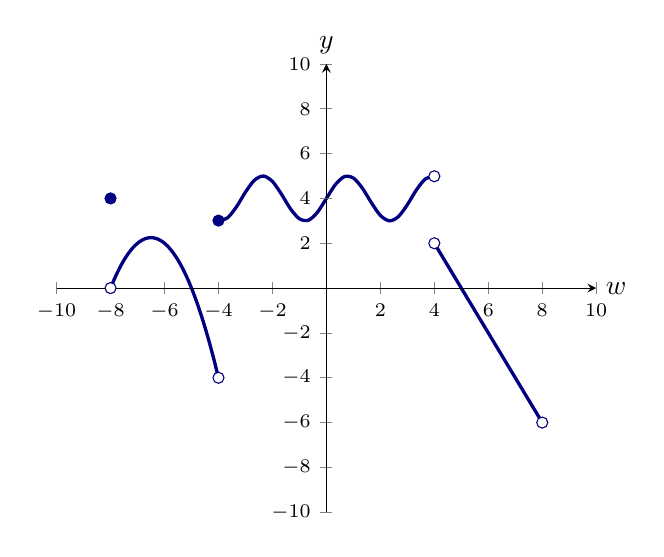
\begin{tikzpicture}
     \begin{axis}[
            	domain=-10:10, ymax=10, xmax=10, ymin=-10, xmin=-10,
            	axis lines =center, xlabel=$w$, ylabel=$y$,
                ytick={-10,-8,-6,-4,-2,2,4,6,8,10},
                xtick={-10,-8,-6,-4,-2,2,4,6,8,10},
                yticklabels={$-10$,$-8$,$-6$,$-4$,$-2$,$2$,$4$,$6$,$8$,$10$}, 
                xticklabels={$-10$,$-8$,$-6$,$-4$,$-2$,$2$,$4$,$6$,$8$,$10$},
                ticklabel style={font=\scriptsize},
            	every axis y label/.style={at=(current axis.above origin),anchor=south},
            	every axis x label/.style={at=(current axis.right of origin),anchor=west},
            	axis on top,
          		]

        
        \addplot [draw=penColor, very thick, smooth, domain=(-8:-4)] {-(x+8)*(x+5)};
        \addplot [draw=penColor, very thick, smooth, domain=(-4:4)] {sin(deg(2*x)) + 4};
        \addplot [draw=penColor, very thick, smooth, domain=(4:8)] {-2*x+10};


        \addplot[color=penColor,fill=white,only marks,mark=*] coordinates{(-8,0)};
        \addplot[color=penColor,fill=white,only marks,mark=*] coordinates{(-4,-4)};

        \addplot[color=penColor,fill=penColor,only marks,mark=*] coordinates{(-4,3.01) (-8,4)};
        \addplot[color=penColor,fill=white,only marks,mark=*] coordinates{(4,4.989)};

        \addplot[color=penColor,fill=white,only marks,mark=*] coordinates{(4,2)};
        \addplot[color=penColor,fill=white,only marks,mark=*] coordinates{(8,-6)};

    \end{axis}
\end{tikzpicture}
\end{image}








Select all of the discontiuities of $P$.
\begin{selectAll}
\choice [correct]{$-8$}
\choice [correct]{$-4$}
\choice {$-2$}
\choice {$-1$}
\choice {$3$}
\choice {$4$}
\choice {$8$}
\choice {None of the above}
\end{selectAll}





\end{example}







\begin{example} Jump Discontinuity \\

Let $g(k)$ be a function.  The graph of $y= g(k)$ is displayed below. 

\begin{image}
\begin{tikzpicture}
     \begin{axis}[
                domain=-10:10, ymax=10, xmax=10, ymin=-10, xmin=-10,
                axis lines =center, xlabel=$k$, ylabel=$y$,
                ytick={-10,-8,-6,-4,-2,2,4,6,8,10},
                xtick={-10,-8,-6,-4,-2,2,4,6,8,10},
                yticklabels={$-10$,$-8$,$-6$,$-4$,$-2$,$2$,$4$,$6$,$8$,$10$}, 
                xticklabels={$-10$,$-8$,$-6$,$-4$,$-2$,$2$,$4$,$6$,$8$,$10$},
                ticklabel style={font=\scriptsize},
                every axis y label/.style={at=(current axis.above origin),anchor=south},
                every axis x label/.style={at=(current axis.right of origin),anchor=west},
                axis on top,
                ]

        
        \addplot [draw=penColor, very thick, smooth, domain=(-8:-3)] {x};
        \addplot [draw=penColor, very thick, smooth, domain=(-1:4)] {0.5*x+4};
        \addplot [draw=penColor, very thick, smooth, domain=(4:8)] {-2*x+8};


        \addplot[color=penColor,fill=white,only marks,mark=*] coordinates{(-8,-8)};
        \addplot[color=penColor,fill=white,only marks,mark=*] coordinates{(-3,-3)};

        \addplot[color=penColor,fill=penColor,only marks,mark=*] coordinates{(-1,3.5)};
        \addplot[color=penColor,fill=white,only marks,mark=*] coordinates{(4,6)};

        \addplot[color=penColor,fill=penColor,only marks,mark=*] coordinates{(4,0)};
        \addplot[color=penColor,fill=white,only marks,mark=*] coordinates{(8,-8)};
        \addplot[color=penColor,fill=penColor,only marks,mark=*] coordinates{(8,-2)};

        \addplot[color=penColor,fill=penColor,only marks,mark=*] coordinates{(-2, 2)};

    \end{axis}
\end{tikzpicture}
\end{image}


\begin{itemize}
\item $4$ is a discontinuity of $g(k)$.  \\


First, $4$ is in the domain of $g$. \\


For the second condition, let $d = 1$. Any small open interval of real numbers containing $c = 4$ must also contain an interval of the form $(4-\epsilon, 4+\epsilon)$, where $0 < \epsilon < 0.1$.  Such an interval would ALWAYS contain the domain number $e = 4-\frac{\epsilon}{2}$.

\[ \left| g(4) - g\left(4-\frac{\epsilon}{2}\right) \right| >  1 = d \]

Therefore, $4$ is a discontinuity of $g$. \\


\item $-2$ is not a discontinuity of $g$, because we can find an open interval of real numbers that does not contain a domain number different from $-2$.  No matter what $d$ you select, the open interval $(-2.01, -1.99)$ does not contain a different domain number, $e \ne -2$, such that $|g(-2) - g(e)| > d$.  Therefore, the second condition for discontinuities does not hold.  $-2$ is not a discontinuity. \\




\item $8$ is a discontinuity of $g(k)$.  First, $8$ is in the domain of $g$. For the second condition, let $d = 1$. Any small open interval of real numbers containing $c = 8$ must also contain an interval of the form $(8-\epsilon, 8+\epsilon)$, where $0 < \epsilon < 0.1$.   Such an interval would ALWAYS contain the domain number $e = 8-\frac{\epsilon}{2}$.

\[ \left| g(8) - g\left(8-\frac{\epsilon}{2}\right) \right| > 1 = d \]

Therefore, $8$ is a discontinuity of $g$.

\end{itemize}



\end{example}

This is the type of exactness we want in our discussions.  This is \textbf{\textcolor{purple!85!blue}{rigor}}. We want to talk algebraically about ``always'', ``close enough'', and ``small enough''.  Fluency in the notational language will take some time.  But we have some time until Calculus.












\begin{example} Removeable Discontinuity \\

Let $T(y)$ be a function.  The graph of $z = T(y)$ is displayed below. 

\begin{image}
\begin{tikzpicture}
     \begin{axis}[
                domain=-10:10, ymax=10, xmax=10, ymin=-10, xmin=-10,
                axis lines =center, xlabel=$y$, ylabel=$z$,
                ytick={-10,-8,-6,-4,-2,2,4,6,8,10},
                xtick={-10,-8,-6,-4,-2,2,4,6,8,10},
                yticklabels={$-10$,$-8$,$-6$,$-4$,$-2$,$2$,$4$,$6$,$8$,$10$}, 
                xticklabels={$-10$,$-8$,$-6$,$-4$,$-2$,$2$,$4$,$6$,$8$,$10$},
                ticklabel style={font=\scriptsize},
                every axis y label/.style={at=(current axis.above origin),anchor=south},
                every axis x label/.style={at=(current axis.right of origin),anchor=west},
                axis on top,
                ]

        
        \addplot [draw=penColor, very thick, smooth, domain=(-8:-3)] {x};
        \addplot [draw=penColor, very thick, smooth, domain=(-1:4)] {0.5*x+4};
        \addplot [draw=penColor, very thick, smooth, domain=(4:8)] {-2*x+8};


        \addplot[color=penColor,fill=white,only marks,mark=*] coordinates{(-8,-8)};
        \addplot[color=penColor,fill=white,only marks,mark=*] coordinates{(-3,-3)};

        \addplot[color=penColor,fill=penColor,only marks,mark=*] coordinates{(-1,3.5)};
        \addplot[color=penColor,fill=white,only marks,mark=*] coordinates{(4,6)};

        \addplot[color=penColor,fill=penColor,only marks,mark=*] coordinates{(4,0)};
        \addplot[color=penColor,fill=white,only marks,mark=*] coordinates{(8,-8)};

        \addplot[color=penColor,fill=white,only marks,mark=*] coordinates{(-6,-6)};
        \addplot[color=penColor,fill=penColor,only marks,mark=*] coordinates{(-6,-3)};
        \addplot[color=penColor,fill=white,only marks,mark=*] coordinates{(7,-6)};

    \end{axis}
\end{tikzpicture}
\end{image}

\begin{itemize}
\item $7$ is not a discontinuity of $T$, because $7$ is not a member of the domain of $T$. ($7$ is a singularity.) \\

\item $-6$ is a discontinuity of $T(y)$.  $-6$ is in the domain of $T$.  For the second condition, let $d = 0.5$. Any small open interval of real numbers containing $c = -6$ must also contain an interval of the form $(-6-\epsilon, -6+\epsilon)$, where $0 < \epsilon < 0.1$.   Such an interval would ALWAYS contain the domain number $e = -6+\frac{\epsilon}{2}$.

\[ \left| T(-6) - T\left(-6+\frac{\epsilon}{2}\right) \right| > 1 > 0.5 = d \]

Therefore, $-6$ is a discontinuity of $T$. \\


\item $4$ is a discontiuity of $T(y)$.   $4$ is in the domain of $T$.  For the second condition, let $d = 0.5$. Any open interval of real numbers containing $c = 4$ must also contain an interval of the form $(4-\epsilon, 4+\epsilon)$, where $0 < \epsilon < 0.1$.   Such an interval would ALWAYS contain the domain number $e = 4-\frac{\epsilon}{2}$.

\[ \left| T(4) - T\left(4-\frac{\epsilon}{2}\right) \right| > 1 > 0.5 = d \]

Therefore, $4$ is a discontinuity of $T$. \\

\end{itemize}



\end{example}

No matter how close you get to $-6$ in the domain, there is ALWAYS a jump of more than $1$ in the value of the function.  \\










\begin{example} Asymptotic Discontinuity \\

Let $f(x)$ be a function.  The graph of $y = f(x)$ is displayed below. 



\begin{image}
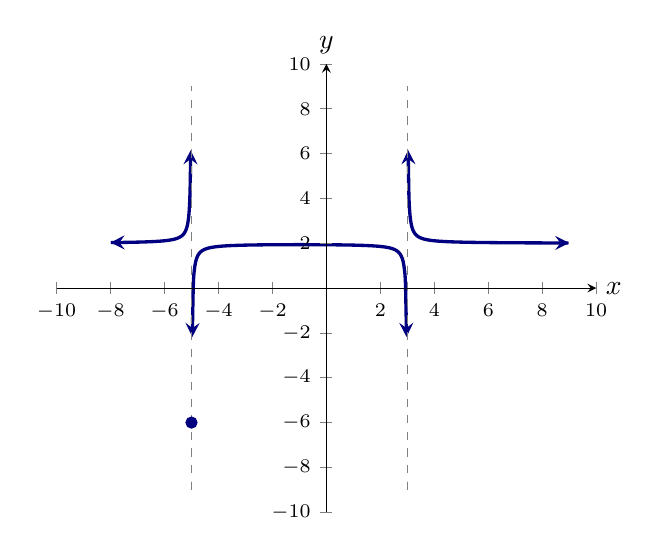
\begin{tikzpicture}
     \begin{axis}[
                domain=-10:10, ymax=10, xmax=10, ymin=-10, xmin=-10,
                axis lines =center, xlabel=$x$, ylabel=$y$,
                ytick={-10,-8,-6,-4,-2,2,4,6,8,10},
                xtick={-10,-8,-6,-4,-2,2,4,6,8,10},
                yticklabels={$-10$,$-8$,$-6$,$-4$,$-2$,$2$,$4$,$6$,$8$,$10$}, 
                xticklabels={$-10$,$-8$,$-6$,$-4$,$-2$,$2$,$4$,$6$,$8$,$10$},
                ticklabel style={font=\scriptsize},
                every axis y label/.style={at=(current axis.above origin),anchor=south},
                every axis x label/.style={at=(current axis.right of origin),anchor=west},
                axis on top,
                ]

        
        \addplot [draw=penColor, very thick, smooth, samples=200, domain=(-8:-5.03), <->] {1/((x-3)*(x+5)) + 2};
        \addplot [draw=penColor, very thick, smooth, samples=200, domain=(-4.97:2.97), <->] {1/((x-3)*(x+5)) + 2};
        \addplot [draw=penColor, very thick, smooth, samples=200, domain=(3.03:9), <->] {1/((x-3)*(x+5)) + 2};

        \addplot [line width=0.5, gray, dashed,samples=100,domain=(-9:9)] ({3},{x});
        \addplot [line width=0.5, gray, dashed,samples=100,domain=(-9:9)] ({-5},{x});

        \addplot[color=penColor,fill=penColor,only marks,mark=*] coordinates{(-5,-6)};

    \end{axis}



\end{tikzpicture}
\end{image}

\begin{itemize}
\item $3$ is not a discontinuity of $f$, because $3$ is not a member of the domain of $f$. ($3$ is a singularity.) \\

\item $-5$ is a discontinuity of $f(x)$.  For the second condition, let $d = 0.5$. Any open interval of real numbers containing $c = -5$ must also contain an interval of the form $(-5-\epsilon, -5+\epsilon)$, where $0 < \epsilon < 0.000001$.    Such an interval would ALWAYS contain the domain number $e = -5-\frac{\epsilon}{2}$.

\[ \left| f(-5) - f\left(-5-\frac{\epsilon}{2}\right) \right| > 0.5 = d \]

Therefore, $-5$ is a discontinuity of $f$.

\end{itemize}

\end{example}





\begin{observation} \textbf{\textcolor{blue!55!black}{But, But, But, ...}}  

The example above illustrates that the difference between a real number being a discontinuity or not can be very thin.

This is why we also have the \textit{singularity} category.

\end{observation}










\begin{idea} \textbf{\textcolor{green!50!black}{A Singularity}}  

A real number, $c$, is said to be a \textbf{singularity} of the function $f$, if $c$ is not a member of the domain of $f$, however, $c$ is surrounded by the domain or is an edge of the domain, and the function has extreme/weird/unexpected behavior there. ($c$ is not in the domain, but it wouldn't be a singleton if it were included in the domain.) \\



$\blacktriangleright$  $c$ is not in the domain, however, 


\begin{itemize}
\item EVERY open interval containing $c$ does contain a domain number and 
\item the function is behaving extreme/weird/unexpected near $c$. \\
\end{itemize}
It turns our ``weird'' includes a lot of behavior.  It will take a while to state a \textbf{\textcolor{purple!85!blue}{rigorous}} definition of singularity.  In the mean time, we will keep noting weird behavior and building our feeling of weird.


We will extend and sharpen our ideas and definition of singularity in Calculus.



\end{idea}



















\begin{example} 



Let $h(v)$ be a function.  The graph of $y = h(v)$ is displayed below. 

\begin{image}
\begin{tikzpicture}
     \begin{axis}[
                domain=-10:10, ymax=10, xmax=10, ymin=-10, xmin=-10,
                axis lines =center, xlabel=$v$, ylabel=$y$,
                ytick={-10,-8,-6,-4,-2,2,4,6,8,10},
                xtick={-10,-8,-6,-4,-2,2,4,6,8,10},
                yticklabels={$-10$,$-8$,$-6$,$-4$,$-2$,$2$,$4$,$6$,$8$,$10$}, 
                xticklabels={$-10$,$-8$,$-6$,$-4$,$-2$,$2$,$4$,$6$,$8$,$10$},
                ticklabel style={font=\scriptsize},
                every axis y label/.style={at=(current axis.above origin),anchor=south},
                every axis x label/.style={at=(current axis.right of origin),anchor=west},
                axis on top,
                ]

        
        \addplot [draw=penColor, very thick, smooth, domain=(-8:-3)] {2^(-x-5)};
        \addplot [draw=penColor, very thick, smooth, domain=(-1:5)] {-2*x+4};
        \addplot [draw=penColor, very thick, smooth, domain=(5:8)] {-2};


        \addplot[color=penColor,fill=white,only marks,mark=*] coordinates{(-8,8)};
        \addplot[color=penColor,fill=white,only marks,mark=*] coordinates{(-3,0.25)};

        \addplot[color=penColor,fill=penColor,only marks,mark=*] coordinates{(-1,6)};
        \addplot[color=penColor,fill=white,only marks,mark=*] coordinates{(4,-4)};

        \addplot[color=penColor,fill=penColor,only marks,mark=*] coordinates{(4,6)};
        \addplot[color=penColor,fill=white,only marks,mark=*] coordinates{(5,-2)};

        \addplot[color=penColor,fill=white,only marks,mark=*] coordinates{(5,-6)};
        \addplot[color=penColor,fill=penColor,only marks,mark=*] coordinates{(8,-2)};

    \end{axis}
\end{tikzpicture}
\end{image}





\begin{question}

$4$ is a \wordChoice{\choice[correct]{discontinuity}\choice{singularity}} of $h$.


\end{question}





\begin{question}

$5$ is a \wordChoice{\choice{discontinuity}\choice[correct]{singularity}} of $h$.


\end{question}





\begin{question}

Is $-1$ a discontiuity, sigualrity, or neither of $h$.

\begin{multipleChoice}
\choice {discontinuity}
\choice {singularity}
\choice [correct] {neither}
\end{multipleChoice}


\end{question}







\end{example}






\begin{definition} \textbf{\textcolor{green!50!black}{Continuity}} \\


Let $f$ be a function. \\
If $c$ is in the domain of $f$ and $c$ is not a discontinuity, then $f$ is said to be \textbf{contiuous} at $c$. \\


If $S$ is a subset of the domain and $f$ is continuous at every number in $S$, then $f$ is said to be continuous on the subset. \\

A function that is continuous on its whole domain is just said be a continuous function. \\


\end{definition}




\begin{warning}


A function is not continuous at a singularity, because the singularity is not in the domain.  However, the singularity is not a discontinuity, because the singularity is not in the domain. \\

So, it is possible for a function to be noncontinuous and yet not have discontinuity. 



\end{warning}





\begin{idea} \textbf{\textcolor{blue!55!black}{Continuity}}


Continuous means not discontinuous in the domain. \\

Discontinuous means there was a fixed distance in the range that separated function values no matter how close the domain numbers were. \\

Continuity means this doesn't happen. \\

\begin{explanation}

Let $f$ be a function and $c$ a number in the domain. \\

$f$ is \textbf{continuous} at $c$ if  \\


For every range distance $\epsilon > 0 $, there is a corresponding domain distance $\delta > 0$ such that \\


for all domain numbers $x$ inside $(c - \delta, c + \delta)$ we have $| f(x) - f(c) | < \epsilon$. \\

\end{explanation}

You can get close enough to $c$ in the domain so that all of the function values are close to $f(c)$...as close as you want...any closeness. \\



Continuity: Close in the domain means close in the range.


\end{idea}


As you can see, this is easy to see visually, but difficult to describe algebraically.  It will take some time to describe discontinuities and singularities with algebra.













\begin{center}
\textbf{\textcolor{green!50!black}{ooooo-=-=-=-ooOoo-=-=-=-ooooo}} \\

more examples can be found by following this link\\ \link[More Examples of Visual Features]{https://ximera.osu.edu/csccmathematics/precalculus1/precalculus1/visualFeatures/examples/exampleList}

\end{center}








\end{document}
